\section{Criptografia simétrica}

Algoritmos criptográficos podem ser classificados em \emph{simétricos} e \emph{assimétricos}. Os algoritmos simétricos fornecem propriedades de segurança a partir de um segredo compartilhado, tipicamente chamado de \emph{chave secreta}. Em um contexto de sigilo, chaves de cifração e decifração são idênticas ou podem ser calculadas eficientemente uma a partir da outra. O problema difícil subjacente a esses esquemas costuma ser explorar um espaço de chaves de tamanho gigantesco, em um ataque chamado de \emph{busca exaustiva}. O algoritmo AES (\emph{Advanced Encryption Standard}) é talvez o mais difundido entre os algoritmos simétricos de encriptação em uso, enquanto SHA é uma família padronizada de funções de resumo criptográfico. Algoritmos assimétricos empregam um par de chaves, \emph{pública} e \emph{privada}, que são calculadas de forma a existir uma relação especial entre ambas: calcular a chave pública a partir da chave privada é eficiente, mas não se conhece algoritmo eficiente para resolver o problema no sentido inverso. Assim, a chave pública pode ser utilizada para encriptação ou verificação de assinaturas, sem ameaça à segurança do algoritmo criptográfico, e a chave privada para decriptação ou assinatura digital deve ser mantida em sigilo, sob posse exclusiva do detentor. Criptografia de curvas elípticas (ECC -- \emph{Elliptic Curve Cryptography}) são um exemplo de algoritmo assimétrico.

\subsection{Encriptação}

A propriedade de segurança de \emph{confidencialidade} pode ser fornecida por um par de funções de encriptação $E$ e decriptação $D$, ambas parametrizadas por uma chave $k$. A encriptação de uma mensagem $M$ sob a chave $k$ produz um criptograma $C = E_k(M)$, enquanto a mensagem original pode ser recuperada pela função de decriptação como $M = D_k(C)$, de forma que a propriedade de consistência seja mantida $M = D_k(E_k(M))$ para quaiquer valores de $M$ e $k$.

As funções $E$ e $D$ podem então ser implementadas por um algoritmo simétrico de encriptação de duas formas distintas. \emph{Cifras de bloco}, como o AES, especificam como encriptar uma sequência de \emph{bits} com tamanho fixo, e precisam ser estendidos para mensagens de tamanho arbitrário por meio de um \emph{modo de operação}. \emph{Cifras de fluxo} como ChaCha calculam uma cadeia de chaves a partir da chave $k$, que é então combinada com a mensagem original utilizando operações \texttt{XOR} (OU exclusivo). É desejável que criptogramas transmitidos sob canais de comunicação sejam acompanhados por \emph{autenticadores}, que permitem ao destinatário detectar a outra parte como origem legítima da mensagem e verificar sua integridade.

Há muitos paradigmas diferentes para se construir cifras simétricas. Em geral, os algoritmos seguem a idéia proposta por Shannon~\cite{Shannon49} de um \emph{produto iterado de cifras}, em que uma \emph{função de rodada} composta por cifras menores e parametrizada por \emph{chaves de rodada} é repetida um número fixo $r$ de vezes. A função de rodada combina pequenas \emph{cifras de substituição}, que substituem símbolos para confundir a relação entre o criptograma e a chave criptográfica, com uma \emph{cifra de transposição}, que altera a ordem dos \emph{bits} para espalhar a redundância do texto claro ao longo do criptograma. O cálculo de chaves de rodada $k_i$ a partir da chave $k$ é também chamado de \emph{escalonamento de chaves}.

Os paradigmas clássicos mais comuns para construção de cifras de bloco são \emph{Redes de Feistel} e \emph{Redes de Substituição-Permutação} (SPN -- \emph{Substitution-Permutation Network}). Redes de Feistel (ou cifras de Luby-Rackoff~\cite{LubyR88} utilizam uma função de rodada não-inversível $f$ que atua sobre o bloco de texto claro $(L_0 \parallel R_0)$. A cada rodada, a função $f$ calcula a próxima metade do estado interno pela regra $R_{i+1} = L_i \oplus f(R_i, k_i)$, enquanto a metade restante é uma simples cópia $L_{i+1} = R_i$, até que seja atingido o bloco de criptograma $(L_r \parallel R_r)$. A decriptação segue processo análogo, utilizando as regras inversas $R_{i} = L_{i+1}$ e $L_{i+1} = R_{i+1} \oplus f(L_{i+1}, k_i)$. SPNs alternam \emph{caixas de substituição} que operam sobre pedaços de $\ell$ \emph{bits} do texto claro (que implementam cifras de substituição) com uma \emph{camada de difusão linear} que opera sobre todo o estado interno. Ao final de cada rodada, a chave de rodada $k_i$ é adicionada ao estado interno por uma operação \texttt{XOR}. A decriptação é realizada pela aplicação de operações inversas também na ordem inversa.

Cifras de fluxo, por sua vez, possuem construções derivadas de geradores pseudo-aleatórios, onde a chave criptográfica faz o papel da semente que termina expandida como uma cadeia de chave pseudo-aleatória muito mais longa. Estas devem ser construídas de modo a maximizar o período do gerador, para evitar repetição na cadeia de chaves. Pode-se dizer que cifras de fluxo são um relaxamento do \emph{one-time pad} (OTP), onde cada símbolo do texto claro é combinado com um símbolo aleatório da chave, que deve possuir o mesmo tamanho da mensagem a ser encriptada. A cadeia de chave pseudo-aleatória de uma cifra de fluxo abre mão da \emph{segurança incondicional} do OTP, em favor de introduzir uma premissa computacional para ganho de eficiência.

\subsubsection*{Modos de operação}

Modos de operação podem fornecer apenas confidencialidade para mensagens de tamanho arbitrário ou propriedades de segurança adicionais, como \emph{cifração autenticada} em um único passo. Estes modos dividem a mensagem $M$ em $n$ blocos de mesmo tamanho $\{M_1, \ldots, M_n\}$ e utilizam uma regra para produzir os blocos de criptograma $C = \{C_1, \ldots, C_n\}$.
O último bloco precisa ser completado com \emph{preenchimento} (ou \emph{padding}) para poder ser processado corretamente.
Diversos modos de operação já foram padronizados por agências de padronização como o NIST para utilização governamental ou na indústria, dentre eles CBC, CTR e GCM.

No modo de operação CBC (\emph{Cipher Block Chaining}), o próximo bloco de criptograma é calculado a partir de um bloco de texto claro e o bloco de criptograma anterior, pela regra $C_i = E_k(M_i \oplus C_{i-1})$, para $2 \leq i \leq n$. O bloco $C_0$ é definido como um \emph{vetor de inicialização} $IV$ único e imprevisível, que não deve se repetir ao longo de encriptações distintas. Observe que o encadeamento da encriptação aleatoriza o bloco de texto claro antes da próxima encriptação, fazendo com que blocos idênticos produzem blocos distintos no criptograma. Como apenas a decifração de blocos distintos pode ser feita de modo independente, paralelismo pode ser extraído apenas no processo de decifração.

O modo de operação CTR (\emph{Counter} simula uma cifra de fluxo a partir de uma cifra de bloco. Os blocos do criptograma são calculados pela operação \texttt{XOR} entre blocos de texto claro e encriptação de valores consecutivos do vetor de inicialização $IV$. Portanto, a regra é dada por $C_i = M_i \oplus E_k(IV + i)$, para $1 \leq i \leq n$. Como o processamento de cada bloco é independente, este modo de operação oferece paralelismo tanto na cifração quanto decifração, sendo tipicamente mais eficiente que o modo CBC.

O modo de cifração autenticada \emph{GCM} (\emph{Galois/Counter Mode}) utiliza o modo CTR para cifração e atualiza um autenticador calculado a partir dos blocos de criptograma $C_i$ que permite detectar posteriormente qualquer manipulação do criptograma em trânsito, com alta probabilidade. Opcionalmente, o modo também autentica dados associados transmitidos às claras, funcionalidade útil para autenticar cabeçalhos de pacotes de rede ou outra informação pública cuja integridade deva ser preservada e possa ser verificada pelo destinatário.

\subsection{Funções de \emph{hash} ou resumo criptográfico}

O objetivo de funções de \emph{hash} ou resumo criptográfico é mapear uma cadeia de \emph{bits} de tamanho arbitrário em um \emph{resumo} com tamanho fixo em \emph{bits}. Este resumo tem como papel identificar unicamente a mensagem de entrada, servindo como uma espécie de ``impressão digital''da mesma. São muitas as aplicações em Criptografia e Segurança Computacional de funções criptográficas: armazenamento seguro de senhas, esquemas de assinatura digital, verificação de integridade, derivação de chaves criptográficas, geração de números pseudo-aleatórios, projeto de cifras de fluxo e autenticadores, provas de trabalho de moedas criptográficas, entre outras. A Figura~\ref{fig:hash} apresenta essa funcionalidade abstrata de funções de resumo criptográfico.

\begin{figure}
\begin{center}
    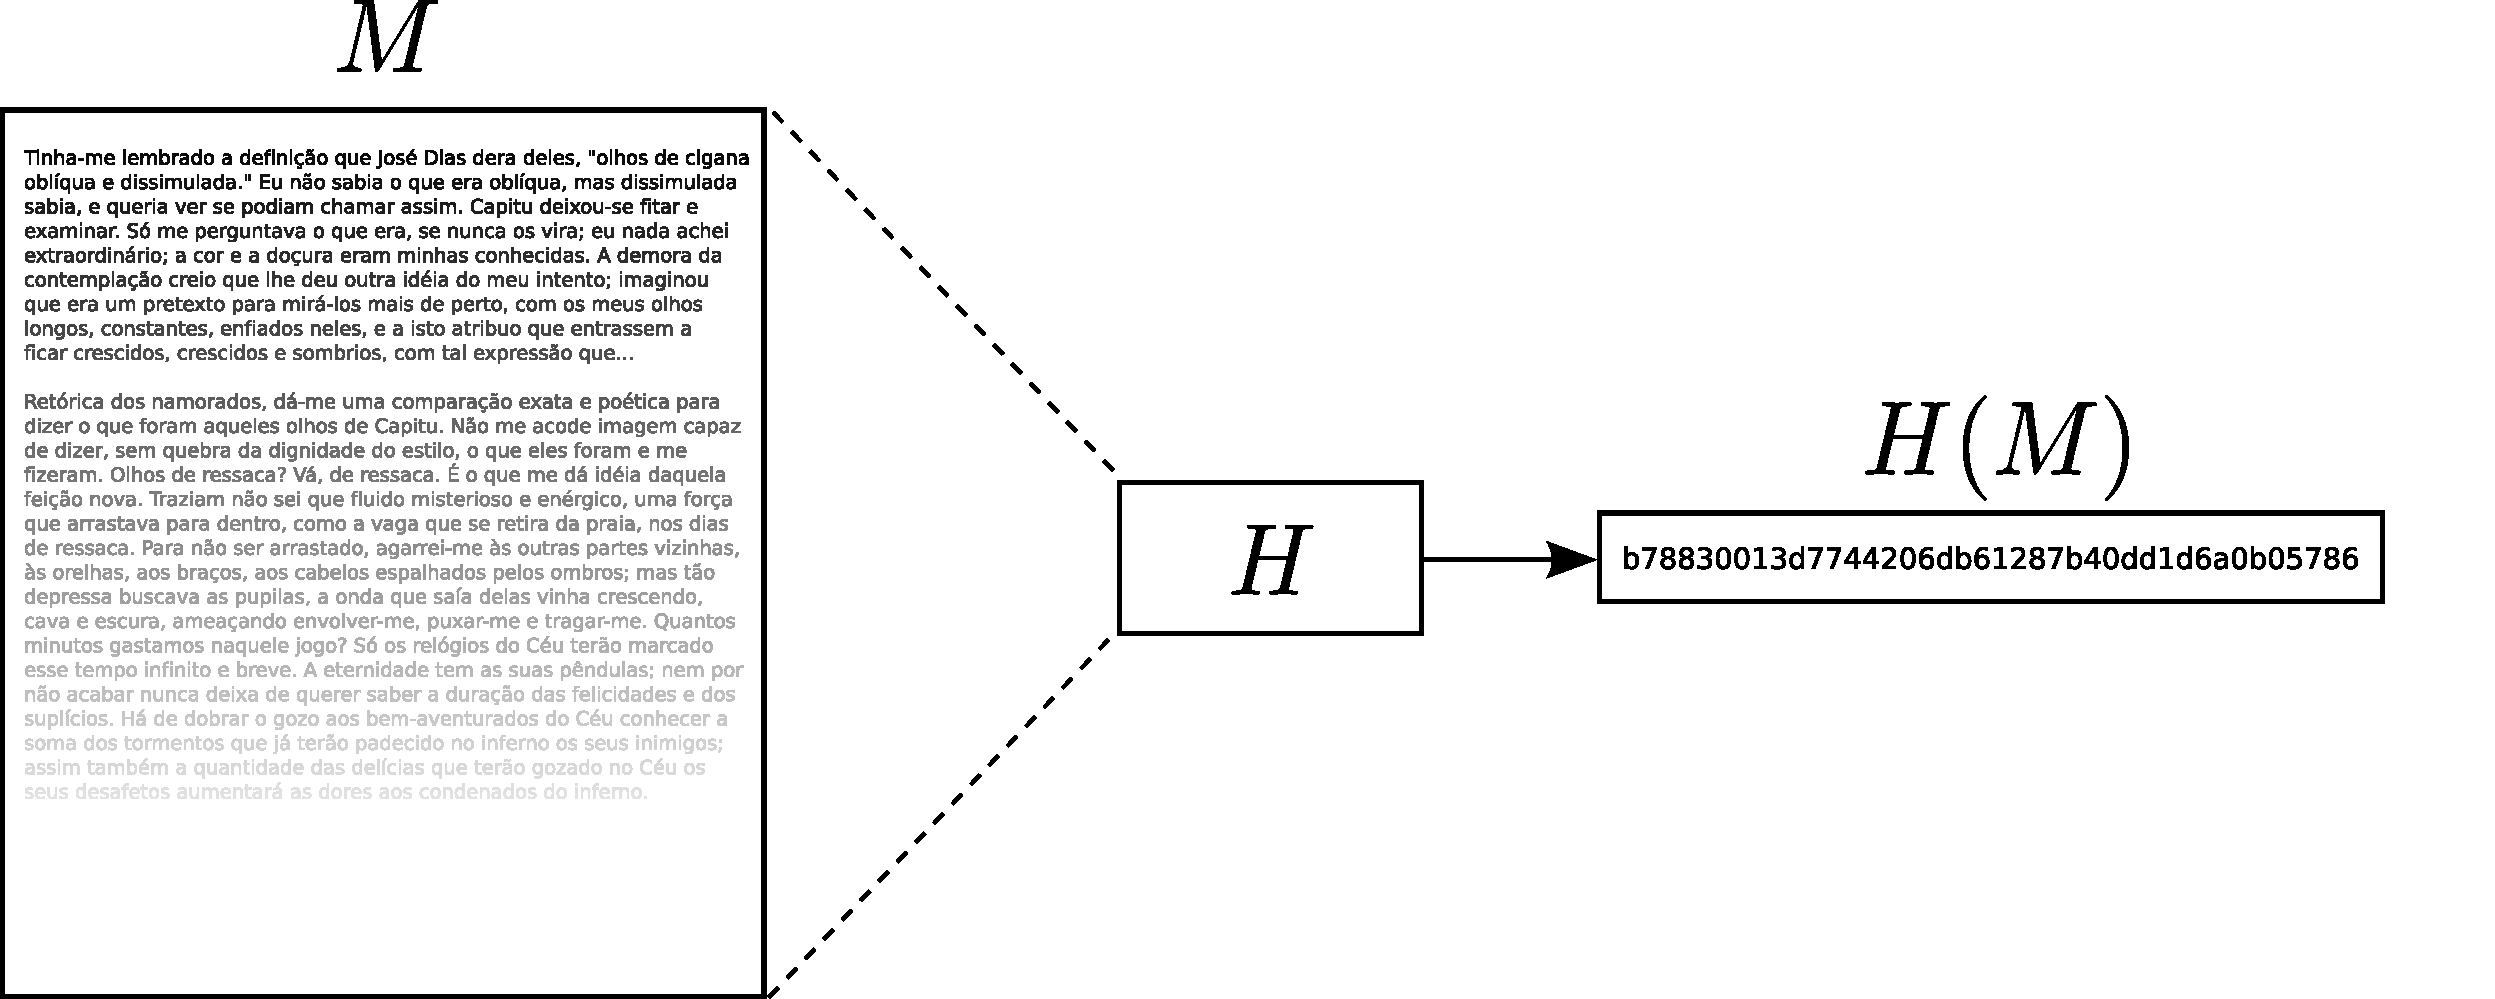
\includegraphics[scale=0.25]{figures/hash.pdf}
    \caption{Função de resumo criptográfico mapeando mensagem $M$ para valor de resumo $H(M)$.}
    \label{fig:hash}
\end{center}
\end{figure}

Em termos matemáticos, funções de resumo são da forma $H : \{0,1\}^* \rightarrow \{0,1\}^n$. Ou seja, mapeiam uma pré-imagem $x$ de tamanho finito e arbitrário em um \emph{valor de hash} $y = H(x)$ de tamanho fixo. A princípio, tratam-se de funções não-chaveadas, ou seja, não-parametrizadas por uma chave criptográfica, mas é claro que podem ser utilizadas também para calcular resumos de informação secreta. Para haver interesse criptográfico, funções de resumo precisam satisfazer as três propriedades abaixo:

\begin{itemize}
 \item {\bf Resistência à pré-imagem}: Dada uma função de resumo criptográfico $H$ e um resumo $y$, deve ser computacionalmente inviável encontrar $x$ tal que $y = H(x)$. Em outras palavras, deve ser difícil ``inverter'' a função para um certo valor de resumo.
 \item {\bf Resistência à segunda pré-imagem}: Dado um resumo $y$ e uma mensagem $x$ tais que $y = H(x)$, deve ser computacionalmente inviável encontrar uma mensagem $x' \neq x$ tal que $h(x') = H(x) = y$. Ou seja, deve ser difícil encontrar uma segunda mensagem mapeada para o meso valor de resumo.
 \item {\bf Resistência a colisões}: Deve ser computacionalmente inviável encontrar mensagens $x, x'$ tais que $H(x) = H(x')$; ou ainda, deve ser difícil encontrar duas mensagens que colidem sob $H$ para um mesmo valor de resumo.
\end{itemize}

Há muitas formas diferentes de se construir essas funções.
Observe que, pelo tamanho e natureza dos conjuntos de domínio e imagem, \emph{colisões} entre diferentes entradas sob uma função $h$ necessariamente irão existir. O desafio é projetar uma função que torne computacionalmente inviável encontrar essas colisões, mesmo que seu número seja infinito.
Classicamente, o paradigma Merkle-Damg\aa rd constrói uma função de resumo criptográfico resistente a colisão a partir de uma função de compressão $h$ com entrada de tamanho fixo, também resistente a colisão~\cite{Merkle79,Damgard89a}. Na Figura~\ref{fig:merkle}, a entrada $X$ é dividida entre $B$ blocos, com aplicação de preenchimento para formar o último bloco, e a saída da última função de compressão define o valor de resumo. Funções de resumo podem também ser construídas a partir de cifras de bloco~\cite{PreneelGV93}, ou problemas difíceis de Teoria dos Números, como a fatoração de inteiros.

\begin{figure}
\begin{center}
    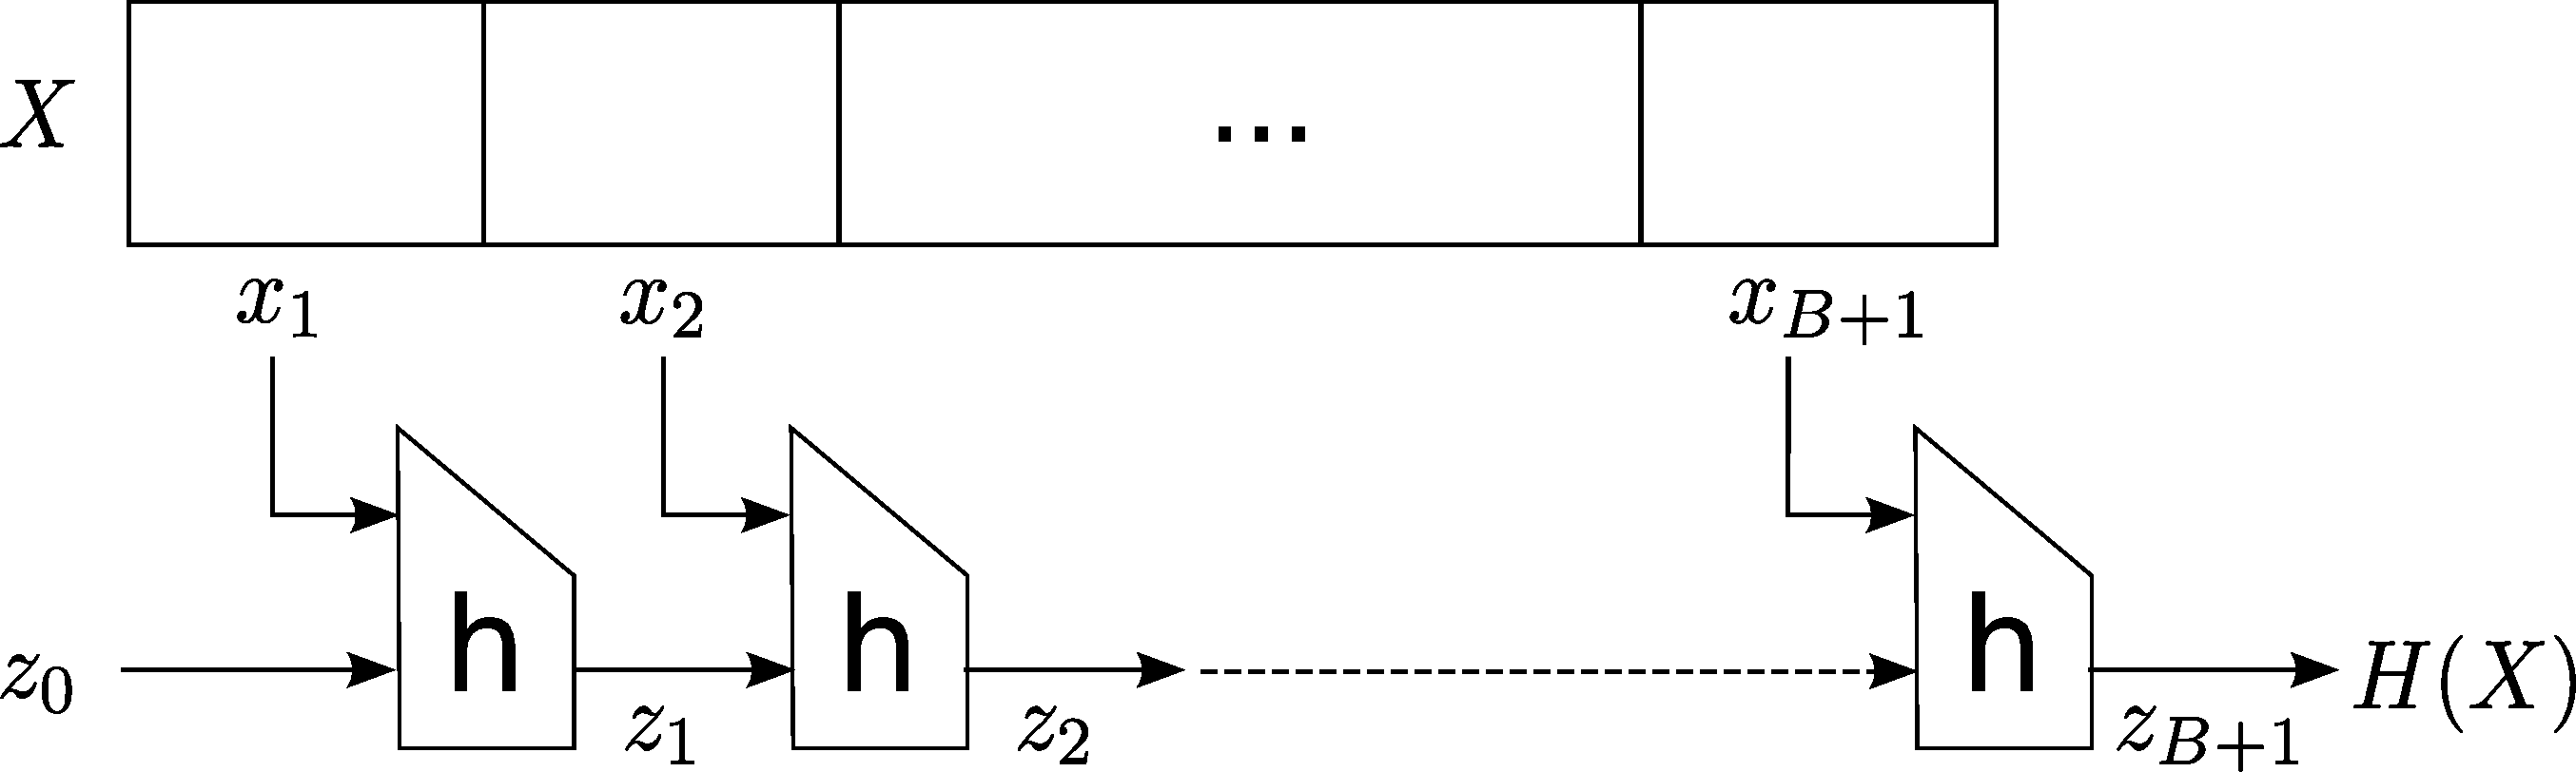
\includegraphics[scale=0.2]{figures/merkle.pdf}
    \caption{Construção Merkle-Damg\aa rd para funções de resumo criptográfico.}
    \label{fig:merkle}
\end{center}
\end{figure}

Um pardigma de construção que se tornou imensamente popular é a classe de \emph{esponjas criptográficas}. Uma esponja é uma função com estado interno $s$ de tamanho finito $b$, dividido em duas seções: a taxa de \emph{bits} de tamanho $r$ e a capacidade de tamanho $c$, tais que $b = c + r$. Completam a especificação uma função de permutação $f$ de tamanho fixo que transforma o estado interno e uma regra de preenchimento. Durante a inicialização, uma função esponja atribui o valor 0 ao estado interno e completa a mensagem de entrada para que seu tamanho seja múltiplo de $r$, de forma que a entrada possa ser dividida em blocos de tamanho $r$. A cada iteração da função, um novo bloco da entrada é adicionado a parte do estado interno pela operação \texttt{XOR} e o estado interno $s$ é substituído por $f(s)$. Em outras palavras, os blocos da entrada são absorvidos sucessivamente no estado interno. Na etapa final, toma-se $r$ bits do estado interno por iteração até que a saída atinja um tamanho pré-determinado, alternando com novas aplicações da função de permutação $f(s)$. A resistência a colisões ou ataques de pré-imagem dependem do tamanho $c$, tipicamente escolhido como duas vezes o nível de segurança desejado. A Figura~\ref{fig:sponge} apresenta a construção~\cite{BertoniDPA08}.

\begin{figure}[h!]
\begin{center}
    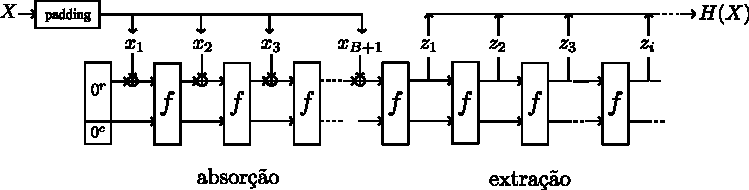
\includegraphics{figures/sponge.pdf}
    \caption{Esponja criptográfica, e suas fases de absorção e extração.}
    \label{fig:sponge}
\end{center}
\end{figure}







